%Correct the file name.
%X: book number
%Y: part number
%ZZZ: page number in three digits. So page 3 would be 003.

\documentclass[11pt]{amsbook}

\usepackage{../HBSuerDemir}	% ------------------------


\begin{document}

% ++++++++++++++++++++++++++++++++++++++
\hPage{Feyzioglu-082}
% ++++++++++++++++++++++++++++++++++++++
\noindent appyling the induction hypothesis to \emph{n-i} with the elements $a_(i+1)$,...,$a_n$, we conclude that $P_n(a_(i+1),...,a_n)$ has one and only one element. This gives $y=t$. Then we get $u=xy=sy=st=v$. So the claim is proved in case $i=j$. \\ \\
\noindent Now suppose $i \neq j$. Without losing generality, we assume $i<j$. We put $j=i+h$, with $ h \in \mathbf N $. Now apply the induction hypothesis to $j$, with the elements $a_1,...,a_j$. There is unique element in $P_j(a_1,...,a_j)$, which we called $s$. Also by induction, applied to $i$ with the elements $a_1,...,a_i$, there is a unique element in $P_i(a_1,a_2,...,a_i)$, namely $x$. Again by induction, applied to $h$ with the elements $a_i_+_1,...,a_j$ there is a unique element in $P_h(a_i_+_1,...,a_j)$, say $b$. By the definition of $P_j(a_1,...,a_j)$, we have $ xb$\in $P_j(a_1,...,a_j)$, so $xb=s$. \\ \\
\noindent We have $n-i=h+(n-j)$. By induction, applied to $n-i$ with the elements $a_i_+_1,...,a_n$, the set $P_n_-_i(a_i_+_1,...,a_n)$ has one and only one element, which we called $y$. Also by induction, applied to $h$ with the elements $a_i_+_1,...,a_j$, there is a unique element in $P_h(a_i_+_1,...,a_j)$, namely $b$. Again by induction, applied to $n-j$ with the elements $a_j_+_1,...,a_n$, the set $P_n_-_j(a_j_+_1,...,a_n)$ has a unique element, namely $t$. By the definition of $P_n_+_i(a_i_+_1,...,a_i_+_h,a_j_+_1,...,a_n)$, we have $bt$ \in $P_n_-_i(a_i_+_1,...,a_n)$, so $bt=y$. \\ \\
\noindent Thus $xb=s$ and $bt=y$. This gives $u=xy=x(bt)=(xb)t=st=v$. This completes the proof. \\ \\ \\ \\
\noindent \textbf{8.4 Definition}  The unique element in $P_n(a_1,a_2,...,a_n)$ of Lemma $8.3$ is called the \emph{product of} $a_1,a_2,...,a_n$ (in this order) and is denoted by $a_1a_2...a_n$ or by \left\prod\limits_{i=1}^n $a_i$. \\ \\
\noindent So the product of \emph{n} elements in a given order can be written without parantheses. This simplifies the notation enormously. \\ \\
\noindent Using the notation of definition 8.4, we can reformulate Lemma 8.3 as follows. If \emph{G} is nonempty set with an associative multiplication on it, and if $a_1,a_2,...,a_n$ \in \emph{G}, then \\ \\
\noindent $a_1(a_2...a_n)=(a_1a_2)(a_3..a_n)=(a_1a_2a_3)(a_4..a_n)=...=(a_1a_2a_3..a_n_-_1)(a_n)=a_1a_2..a_n$







% =======================================================
\end{document}  

%==== templates ====

%==== environments ====

%\begin{figure}[htb]
%	\centering
%	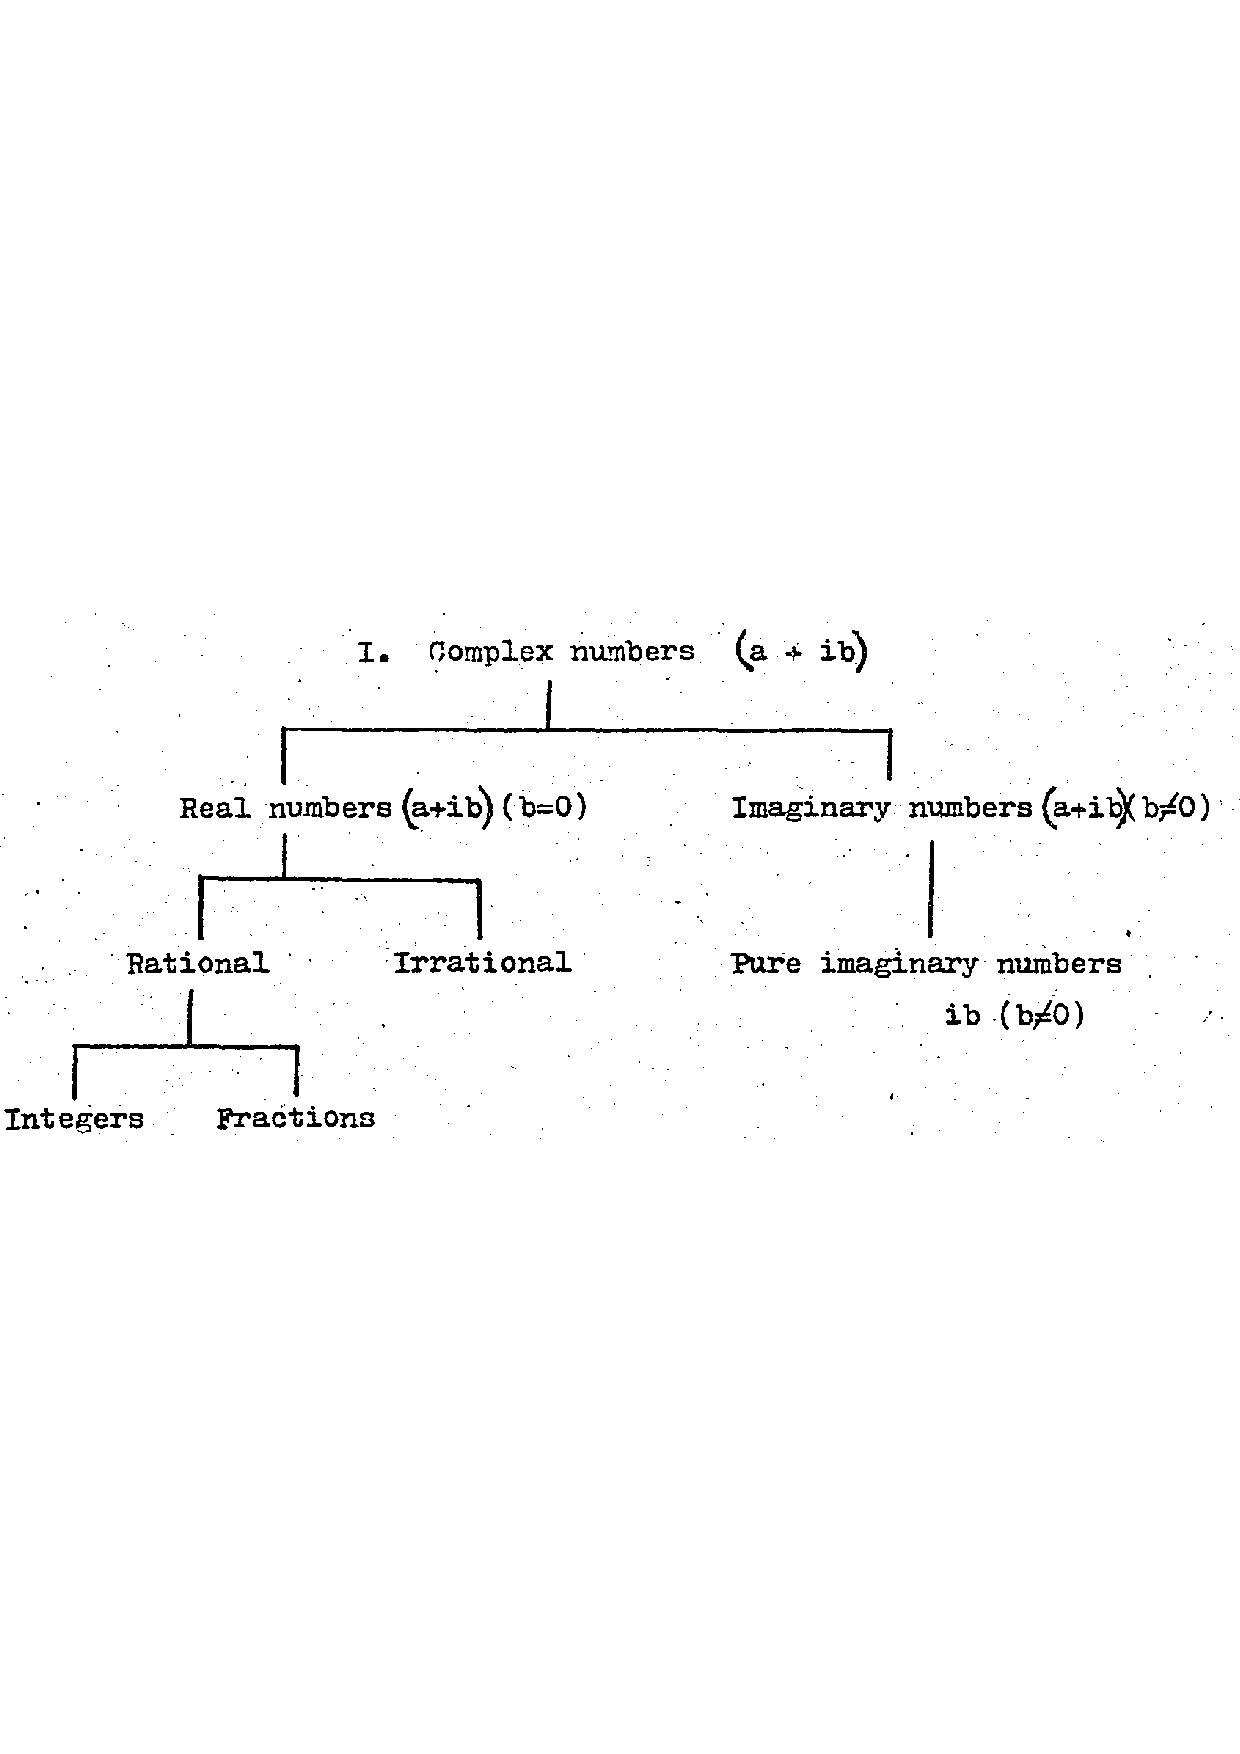
\includegraphics[width=0.9\textwidth]{images/SD-1-1p15A}
%	\caption{Classification of complex numbers}
%	\label{fig:classificationOfComplexNumbersA}
%\end{figure}

%\begin{center}
%\begin{tabular}{cc}
%\end{tabular}
%\end{center}

%\begin{exmp}
%\begin{hSolution}
%\end{hSolution}
%\end{exmp}

%\begin{hEnumerateAlpha}
%\end{hEnumerateAlpha}

%\begin{hEnumerateRoman}
%\end{hEnumerateRoman}

%$
%\begin{bmatrix}
%\end{bmatrix}
%$

%\frac{aaaa}{bbb}
%\frac{a_{n}}{b_{n}}
%\left( aaaa \right)
%\Longrightarrow

%\begin{multicols}{2}
%	bb
%\columnbreak
%	aa
%\end{multicols}
